\documentclass[10pt,twocolumn,letterpaper]{article}

% \usepackage[review]{cvpr}      % To produce the REVIEW version
% \usepackage{cvpr}              % To produce the CAMERA-READY version
\usepackage[pagenumbers]{cvpr} % To force page numbers, e.g. for an arXiv version

% Include other packages here, before hyperref.
\usepackage{graphicx}
\usepackage{amsmath}
\usepackage{amssymb}
\usepackage{booktabs}


% It is strongly recommended to use hyperref, especially for the review version.
% hyperref with option pagebackref eases the reviewers' job.
% Please disable hyperref *only* if you encounter grave issues, e.g. with the
% file validation for the camera-ready version.
%
% If you comment hyperref and then uncomment it, you should delete
% ReviewTempalte.aux before re-running LaTeX.
% (Or just hit 'q' on the first LaTeX run, let it finish, and you
%  should be clear).
\usepackage[pagebackref,breaklinks,colorlinks]{hyperref}
\hypersetup{
   colorlinks=true,
   linkcolor=blue,
   filecolor=magenta,
   urlcolor=cyan,
   citecolor=blue,
}


% Support for easy cross-referencing
\usepackage[capitalize]{cleveref}
\crefname{section}{Sec.}{Secs.}
\Crefname{section}{Section}{Sections}
\Crefname{table}{Table}{Tables}
\crefname{table}{Tab.}{Tabs.}


%%%%%%%%% PAPER ID  - PLEASE UPDATE
\def\cvprPaperID{*****} % *** Enter the CVPR Paper ID here
\def\confName{CVPR}
\def\confYear{2023}


\begin{document}

\title{Co-Citation Prediction with Graph Networks and Transformers}

\author{Samihan Dani, Gaurav Sett\\
Georgia Insitute of Technology\\
\{sdani30, gauravsett\}@gatech.edu
% For a paper whose authors are all at the same institution,
% omit the following lines up until the closing ``}''.
% Additional authors and addresses can be added with ``\and'',
% just like the second author.
% To save space, use either the email address or home page, not both
% \and
% Second Author\\
% Institution2\\
% First line of institution2 address\\
% {\tt\small secondauthor@i2.org}
}
\maketitle


\begin{abstract}
   A vast number of academic papers are published each year. Especially in fast-paced disciplines like computer science, it is impossible for researchers to develop a comprehensive understanding of the landscape. 
   Citation networks have become a dominant approach to understanding the relationships between papers. Co-citation, where two papers are cited together, has been used to track the evolution of research topics. However, this work has been largely descriptive.
   We employ a novel deep learning techniques to predict co-citations.
   Our model is composed of an encoder to represent the semantic information of each paper, a graph network to represent the citation network, and a regression head to predict the number of co-citations for a pair of papers.
\end{abstract}


\section{Introduction}
\label{sec:intro}

Even with advances in search engines and recommendation systems, it is difficult for researchers to keep up with the vast amount of literature published each year. In 2018, 2.6 million papers were published around the world \cite{white2019publications}. While there are varying estimates of how many are read or cited, it appears that a significant and growing portion receives little attention \cite{evans2008electronic}. In fast paced disciplines like computer science, it is impossible for researchers to keep track of all new developments. 

However, the increasing scale of academic literature has been met by a growing number of tools to help researchers parse through the literature. Prior to the internet, researchers were bottlenecked by physical access. Search engines like Google Scholar have also made it much easier to find papers related to key terms. Semantic search, used by platforms like Semantic Scholar, have also improved this process by using machine learning techniques to understand the meaning of a query and the content of a paper. 

In addition to querying papers by topic, researchers also want to find papers that are related in a more nuanced way. Citation networks have become a dominant approach to understanding these relationships, inspired by search algorithms like PageRank \cite{Page1999ThePC}. Citation networks are directed graphs where nodes represent papers and edges represent citations. For decades, researchers have investigated co-citations, where two papers are cited together, to track the evolution of research topics \cite{small1973co}.

Work on co-citation has predominately employed descriptive analysis. However, deep learning techniques give an opportunity to build predictive models. We build a model to predict the likelihood of two papers being co-cited by subsequent work. We use a large language model to encode the semantic information of each paper, a graph convolutional network to incorporate the citation information, and a regression head to predict the number of co-citations expected for a pair of papers.

This work can help researchers manage the depth and breath of academic literature. For example, the model can help identify interdisciplinary research directions, or help consolidate past and present work.

Our code is available at \url{https://github.com/gauravsett/co-citation-prediction}.

\section{Related Work}

The co-citation measure was first introduced in 1973 by Small, taking advantage of newly created scientific citation indices to identify research development and relationships across disciplines \cite{small1973co}. This work has been mostly descriptive, analyzing the structure of academic literature and the usefulness in clustering documents. For example, co-citation has been found to outperform direct citations in the identification of coherent research clusters in biomedicine, but fell short of text-based clustering measures in computer science literature \cite{Boyack2010CocitationAB}. The techniques used to identify co-citation have also evolved. Some studies focus on the co-citation of authors, rather than papers, to identify research communities, and others incorporate temporal modeling \cite{chen2010structure}. 

Some work has used co-citation networks for link prediction. Inspired by PageRank, researchers have used Markov models from these networks to recommended papers \cite{zhu2002using}. Other work has used graph-based growth algorithms to discover subnetworks with a trend of new publications and co-citations \cite{smojver2021exploring}.

However, it appears no work has combined semantic information about paper content with structural information from the citation network to predict co-citation. This work aims to fill the gap using deep learning techniques.

Advances in natural language processing have largely been driven by the development of large language models. These models are trained on large corpora of text to learn the semantic information of language. The most popular of these models are based on transformers, which have been shown to outperform recurrent neural networks \cite{vaswani2017attention}. These models have been used for a variety of tasks, including question answering, text generation, and text classification \cite{devlin2018bert}. These models are encoder-decoder architectures, where the encoder learns the semantic information of the input and the decoder generates the output. The encoder produces a vector representation of the input, which can be used as input to other models. 

The impact of transformers on graph ML has lagged their transformation of natural language processing and computer vision. There are many initiatives to represent graph structures in embeddings for input to transformer models, hoping to leverage their compute efficiency \cite{ying2021transformers,kim2022pure}. However, we aim to leverage both the graph structure of the citation network and semantic information of the paper. The Cascaded Transformers-GNN applies language modeling before the graph modeling \cite{hamilton2017inductive}, while the GraphFormer combines these into an iterative process \cite{yang2021graphformers}. Because we want to prioritize the semantic information for our task, and because we want our embeddings to generalize beyond our paper subset, we privilege the language model in our approach.

Some work has leveraged large language models for link prediction. One  framework called Bi-Link utilizes transformers for link prediction tasks \cite{peng2022bi}. Specifically, they used pre-trained language models to encode textual information about entities and relations in a knowledge graph. They then designed a contrastive learning approach with probabilistic syntax prompts to efficiently search for relational prompts according to learnt syntactical patterns that generalize to large knowledge graphs. This approach allows the model to comprehend the underlying semantics and logic patterns of relations, which is crucial for accurate link prediction.

\section{Data}
\begin{figure}
   \centering
   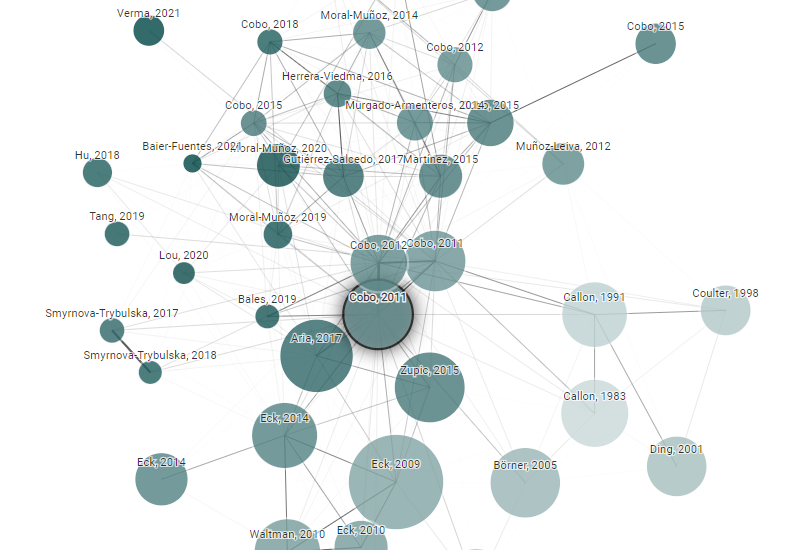
\includegraphics[width=0.5\textwidth]{figures/cit_graph.png}
   \caption{Example of citation graph}
   \label{fig:cite_graph}
\end{figure}

We use the Citation Network Dataset as the basis for our work \cite{tang2008arnetminer}. Specifically, we use the 14th edition of the DBLP citation network collected on January 1st, 2023. DBLP is a large computer science bibliography with 4.4 million publications from 2.2 million authors \cite{ley2002dblp}. A diagram showed in Figure \ref{fig:cite_graph} illustrates how a citation graph should look like. 
For each paper, we have a unique ID, title, author names, publication venue, year, keywords, language, abstract, and most importantly references. These papers date back to 1980.

\begin{table}
   
\end{table}

We filter our dataset for our model. We select only English papers with complete information about abstracts, keywords, venues, and titles. From this set, we selected a random sample of 100,000 papers to reduce computational cost.

For each paper, we constructed a string combining the title, venue, keywords, and abstract to represent the content. This string is later used as input for our encoder model. Our graph model is based on a network where each paper is a node and each citation is an edge drawn from the citing paper to the cited paper. We use the references field to construct this network. 

Some referenced papers from our dataset are not included in our sample. This is a result of the window of the dataset and our sample.
In our graph network, these papers are represented by the average embedding of their neighbors, aiming to reduce the impact of missing data. 
For our regression model, we exclude these examples as we do not have the input data.
However, the random sampling should prevent a selection effect.

\section{Methods}

% (10 points) What did you do exactly? How did you solve the problem? Why did you think it would be successful? Is anything new in your approach?
% (5 points) What problems did you anticipate? What problems did you encounter? Did the very first thing you tried work?

Our approach aims to incorporate both semantic and structural information about papers to predict co-citation. Both intuitively offer important information about how a paper may contribute to literature. Semantic information can help identify topics and subfields. Structural information can represent the attention researchers have paid to different works and the relationships between them. Indeed, this deep learning based approach appears to be novel in the literature. 

\subsection{Architecture}

Our model is composed of three components: an encoder, a graph network, and a regression head. 
The encoder is a language model that encodes the semantic information of each paper. The graph network incorporates the citation network. The regression head predicts the number of co-citations for a pair of papers. We describe each component in detail below.

For our training task, we selected 80\% of co-citation pairs and estimate the number of co-citations for each pair. We use the remaining 20\% of co-citation pairs for validation. 
We use a mean squared error loss function to train our model.
We use the Adam optimizer with a learning rate of 0.00001, a weight decay of 0.001, train for 20 epochs. For our regression task, our batch size is 4096.

\subsubsection{Transformer Encoder}

We use the ``MiniLM-L6-H384-uncased'' language model from the Sentence Transformers library \cite{reimers2019sentence}. This model is based on the BERT architecture \cite{devlin2018bert}. This model has been pre-trained on a large corpus of text and fine-tuned on a 1 billion sentence pairs dataset with a contrastive learning objective. The model outputs a 384-dimensional embedding for each paper.

These embeddings are computed once prior to training and are used as input to the graph network. We do not fine-tune the language model during training.

\subsubsection{Graph Convolutional Network}
\begin{figure}
   \centering
   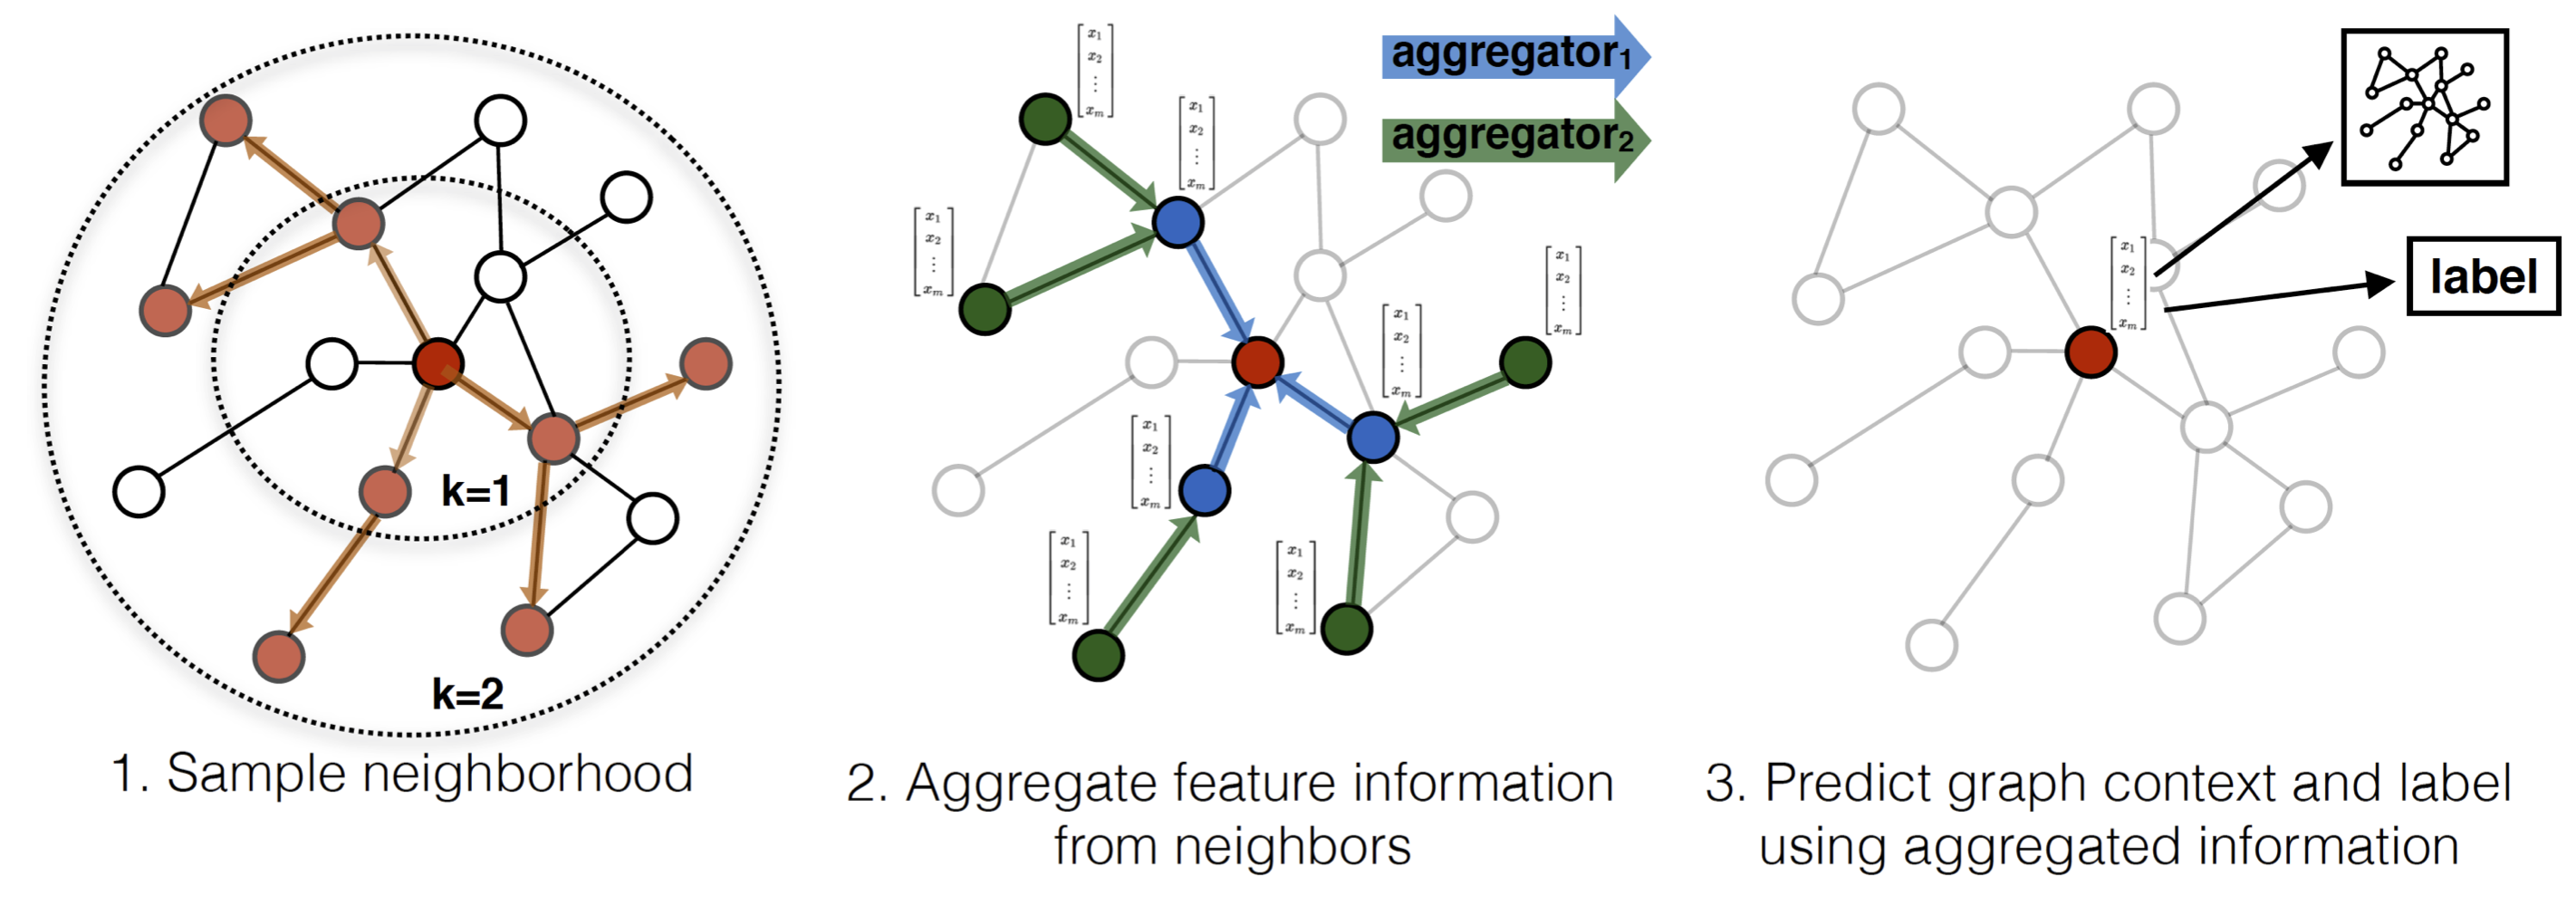
\includegraphics[width=0.5\textwidth]{figures/graphsage.png}
   \caption{Illustration of GraphSAGE Model}
   \label{fig:graph}
\end{figure}

We use a graph convolutional network to incorporate the citation network. We use the PyTorch Geometric library \cite{fey2019fast} to implement this network. Specifically, we use the SageConv layer, which is a graph convolutional layer based on the GraphSAGE algorithm \cite{hamilton2017inductive}. This layer aggregates the embeddings of a node's neighbors and then concatenates this aggregation with it;s own previous embedding. Then, an update function is applied which performs a linear transformation on this vector. For these layers, we use 16 hidden channels, a dropout rate of 0.15, and a ReLU activation function. We apply this layer thrice in the graph network. The number of layers determined the size of the neighborhood for a node's aggregation. For instance, with our implementation, each node aggregates information from every node within a 3-hop radius of the node. This process can be seen in Figure \ref{fig:graph} from \cite{hamilton2017inductive}. 

This model produced convolved embeddings for each paper. We use these embeddings as input to the regression head.

\subsubsection{Regression Head}

Our regression head takes in a concatenated pair of convolved embeddings.
The module is composed of a fully connected layer with a output dimension of 32, a ReLU activation function, and a final fully connected layer with a single output. This output is the predicted number of co-citations for a pair of papers.


\section{Results}

% (10 points) How did you measure success? What experiments were used? What were the results, both quantitative and qualitative? Did you succeed? Did you fail? Why? Justify your reasons with arguments supported by evidence and data. Make sure to mention any code repositories and/or resources that you used!

\begin{figure}
      \centering
      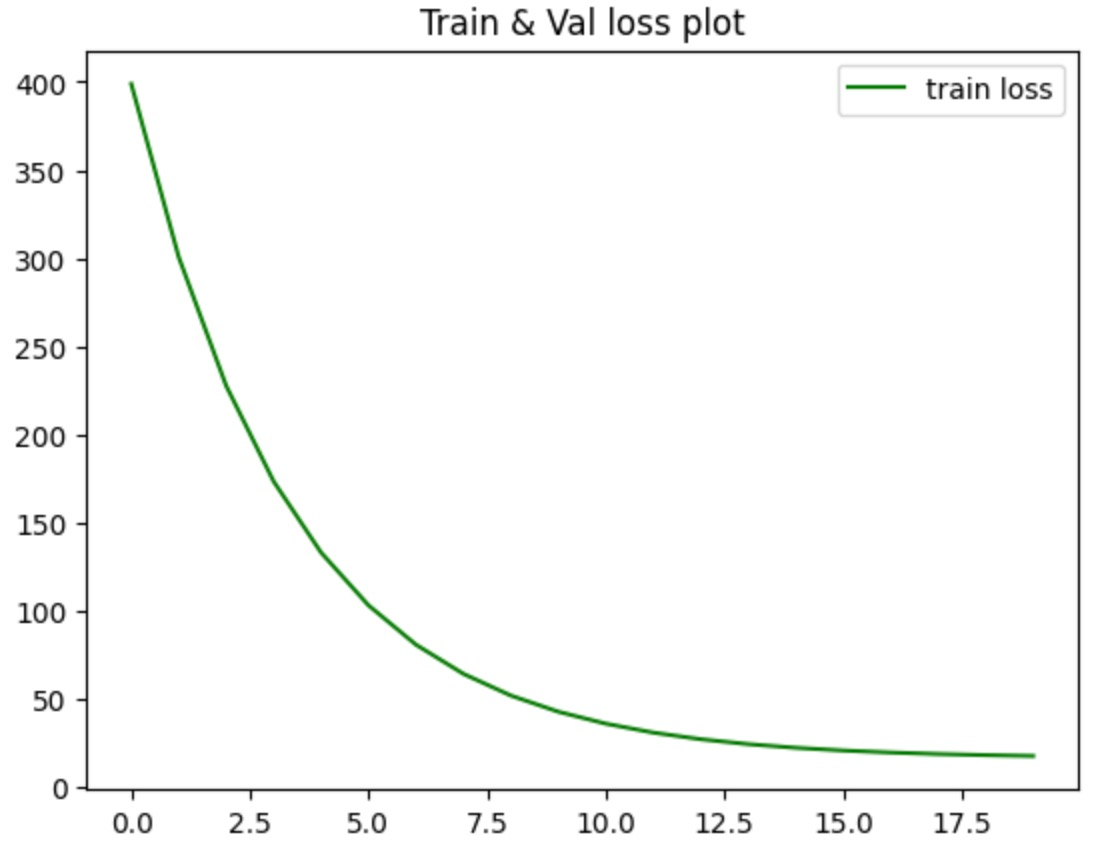
\includegraphics[width=0.5\textwidth]{figures/train-loss.jpeg}
      \caption{Training loss over epochs.}
      \label{fig:train_loss}
\end{figure}

\begin{figure}
   \centering
   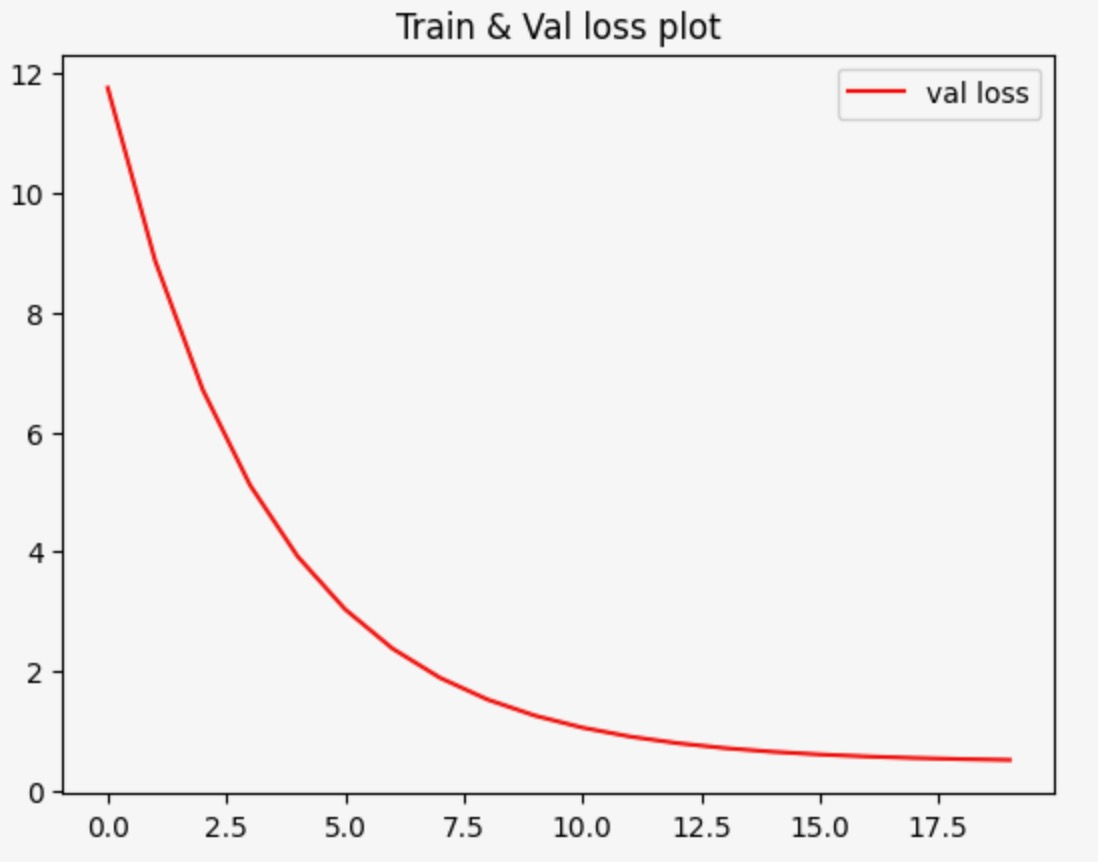
\includegraphics[width=0.5\textwidth]{figures/val-loss.jpeg}
   \caption{Validation loss over epochs.}
   \label{fig:val_loss}
\end{figure}

Our train loss can be seen in Figure \ref{fig:train_loss}. Our validation loss can be seen in Figure \ref{fig:val_loss}. We see that our validation loss plateaus after 10 epochs, suggesting that our model is not learning much after this point.

We evaluate our regression output using $RSME$ and $R^2$. We find that our model has an $RSME$ of 1.145 and an $R^2$ of 0.002. This suggests that our model is not able to predict the number of co-citations well. 

The decrease in our validation loss suggests our model is not overfitting. Upon investigating our model, we find that the model converging on a safe solution of predicting the average number of co-citations. These findings are robust to our tuning of optimizers, learning rates, batch sizes, and hidden dimensions. We also experimented with different architectures for our regression head, changing the number of fully connected layers and the activation functions. 

When removing our encoder model, model performance decreases significantly. This indicates the encoder is successfully capturing semantic information relevant to the task. 

When removing our graph convolutions, model performance slightly decreases. This indicates that the graph network is capturing structural information relevant to the task. 

While this may lead us to believe the regression head is at issue, the model's failure may also be a combination of the encoder and graph network. 


\section{Discussion}

This paper employs a deep learning approach to predict co-citation. We start with a transformer encoder to capture the semantic information of each paper. We then use a graph convolutional network to incorporate the citation network. Finally, we use a regression head to predict the number of co-citations for a pair of papers. 

We find that our model is not able to predict the number of co-citations well. This may be due to the complexity of the task. Co-citation is a complex phenomenon that is not well understood. Additionally, the number of co-citations is a noisy measure of the relationship between papers. For example, a paper may be cited for a variety of reasons, including criticism. We were also limited to paper abstracts which may not contain enough information for the task. 

One additional problem may be that the dataset did not include embeddings for all of the papers referenced. Since we gave these embeddings, the average of all of the existing paper embeddings, it could be that they drowned out the notable papers during the aggregation in the convolutional layer. This explanation aligns with our results since the model seems to predict similar values regardless of the pairs shown. 

Our work should be understood in the context of its limitations. First, our dataset is predominately computer science papers. Amongst those, we have filtered for English language papers only. Additionally, language model capabilities are known to change dramatically at different scales, so our findings may not generalize to other pre-trained encoders.

Future work may investigate different data, pre-trained encoders, and graph network architectures. Additionally, future work may investigate different tasks, such as classification or link prediction.

\section*{Team Contributions}

\textbf{Samihan Dani} contributed to the model implementation, training, and evaluation. He also contributed to the writing of the literature review, methods, and results.

\textbf{Gaurav Sett} contributed to the collection and processing of data and the setup of model pipeline. He also contributed to the writing of the introduction, literature review, data section, and discussion.


%%%%%%%%% REFERENCES
{\small
\bibliographystyle{ieee_fullname}
\bibliography{egbib}
}

\end{document}
